\usetikzlibrary{arrows}
\usetikzlibrary{automata}
\usetikzlibrary{positioning}
\usetikzlibrary{backgrounds}
\usetikzlibrary{fit}

\tikzset{
    state/.style={
           rectangle,
           rounded corners,
           draw=black, very thick,
           minimum height=0.6cm,
           minimum width=1cm,
           inner sep=3pt,
           text centered,
           node distance=0.9cm,
           },
    process/.style={
           rectangle,
           rounded corners,
           draw=black, very thick,
           minimum height=0.6cm,
           minimum width=1cm,
           inner sep=3pt,
           text centered,
           %node distance=1cm,
           },
    newprocess/.style={
           rectangle,
           rounded corners,
           draw=black, very thick,
           fill=lightgray,
           minimum height=0.6cm,
           minimum width=1cm,
           inner sep=3pt,
           text centered,
           %node distance=1cm,
           },
    processplaceholder/.style={
           minimum height=0.6cm,
           minimum width=1cm,
           %inner sep=3pt,
           text centered,
           %node distance=1cm,
           },
    closerstate/.style={
           rectangle,
           rounded corners,
           draw=black, very thick,
           minimum height=0.5cm,
           minimum width=5.32cm,
           inner sep=3pt,
           text centered,
           node distance=1cm,
           },
    abovish/.style={
           rectangle,
           rounded corners,
           draw=none,
           minimum width=1cm,
           text centered,
           node distance=1cm,
           },
    supercloserstate/.style={
           rectangle,
           draw=none,
           minimum height=0.2cm,
           minimum width=6.9cm,
           node distance=1cm,
           },
}

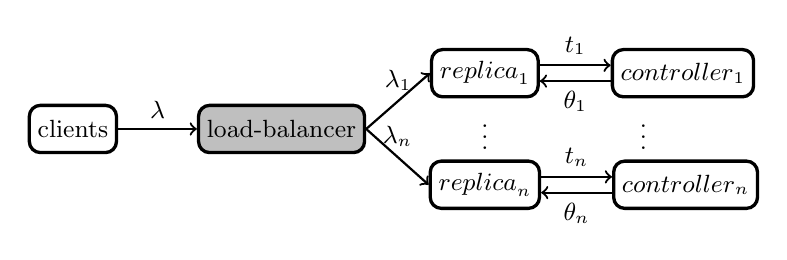
\begin{tikzpicture}[font=\small]
  \tikzstyle{surround} = [fill=black!20,very thick,draw=black,rounded
  corners, inner sep=5pt,] \tikzstyle{surroundblue} =
  [fill=blue!20,very thick,draw=black,rounded corners, inner sep=5pt,]
  \tikzstyle{surroundyellow} = [fill=yellow!20,very
  thick,draw=black,rounded corners, inner sep=5pt,]
  \tikzstyle{external} = [fill=none,very thick,draw=black,rounded
  corners, inner sep=15pt,]

% clients
\node[process] (clients){clients};

% load-balancer
\node[newprocess, right=1cm of clients] (lb){load-balancer};

% servers
\node[processplaceholder, right=1cm of lb] (replicaI) {$\vdots$};
\node[process, above=0cm of replicaI] (replica1) {$\text{replica}_1$};
\node[process, below=0cm of replicaI] (replicaN) {$\text{replica}_n$};

% controllers
\node[processplaceholder, right=1cm of replicaI] (controllerI) {$\vdots$};
\node[process, right=0.9cm of replica1] (controller1) {$\text{controller}_1$};
\node[process, right=0.9cm of replicaN] (controllerN) {$\text{controller}_n$};

% clients to lb
\draw[thick,->] (clients.east) -- (lb.west) node[midway, above] {$\lambda$};

% lb to replicas
\draw[thick,->] (lb.east) -- (replica1.west) node[midway, above] {$\lambda_1$};
\draw[thick,->] (lb.east) -- (replicaN.west) node[midway, above] {$\lambda_n$};

% replica to controllers
\draw[thick,->] ([yshift=+1mm]replica1.east) -- ([yshift=+1mm]controller1.west) node[midway, above] {$t_1$};
\draw[thick,<-] ([yshift=-1mm]replica1.east) -- ([yshift=-1mm]controller1.west) node[midway, below] {$\theta_1$};
\draw[thick,->] ([yshift=+1mm]replicaN.east) -- ([yshift=+1mm]controllerN.west) node[midway, above] {$t_n$};
\draw[thick,<-] ([yshift=-1mm]replicaN.east) -- ([yshift=-1mm]controllerN.west) node[midway, below] {$\theta_n$};

\end{tikzpicture}
